% =============================================================================
% Deep Learning for Parameter Estimation in Spatial Point Processes
% RESTRUCTURING PASS -- no prose has been rewritten, only moved.
%
% HOW TO READ THIS FILE
%   * Every section opens with a % NOTE block stating its PURPOSE and its TODOs.
%   * \todo{...} marks inline gaps (renders red while \drafttrue).
%   * Text carried over from the old draft is tagged % [MOVED FROM: ...].
%   * Sections 2, 7.1, 7.3, 8, 9 are currently empty skeletons -- these are the
%     writing targets. Sections 5 and 6 are largely done.
% =============================================================================

\documentclass[11pt,letterpaper]{article}

\usepackage[margin=1in]{geometry}
\usepackage{mathpazo}

\usepackage{amsmath}
\usepackage{amssymb}
\usepackage{amsthm}
\usepackage{mathtools}
\usepackage{dsfont}

\usepackage{graphicx}
\graphicspath{{../figs/}}
\usepackage{booktabs}
\usepackage{enumitem}

\usepackage{natbib}
\usepackage{xcolor}
\usepackage[hidelinks]{hyperref}

% ----------------------------------------------------------------------------
% Macros (unused ones from the AAAI draft have been deleted)
% ----------------------------------------------------------------------------
\newcommand{\R}{\mathbb{R}}
\newcommand{\N}{\mathbb{N}}
\newcommand{\Z}{\mathbb{Z}}
\newcommand{\E}{\mathbb{E}}
\newcommand{\1}{\mathds{1}}
\newcommand{\pc}{\mathbf{x}}
\newcommand{\simpcom}{\Sigma}
\newcommand{\filt}{\mathcal{F}}
\newcommand{\kpar}{\kappa}
\newcommand{\mo}{\mu}

% ----------------------------------------------------------------------------
% Draft annotations
%   \todo -- prose to write            (red)
%   \fix  -- proposed replacement text (blue)
%   \tab  -- TABLE required here       (green)
%   \fig  -- FIGURE required here      (magenta)
%   \expt -- EXPERIMENT required to support the claim above (orange)
%            (named \expt, not \exp, since \exp is LaTeX's built-in
%            exponential-function operator)
% ----------------------------------------------------------------------------
\newif\ifdraft
\drafttrue
\ifdraft
  \newcommand{\todo}[1]{\textcolor{red}{[TODO: #1]}}
  \newcommand{\fix}[1]{\textcolor{blue}{[FIX: #1]}}
  \newcommand{\tab}[1]{\textcolor{teal}{\textbf{[TABLE:] }#1}}
  \newcommand{\fig}[1]{\textcolor{magenta}{\textbf{[FIGURE:] }#1}}
  \newcommand{\expt}[1]{\textcolor{orange}{\textbf{[EXPT:] }#1}}
\else
  \newcommand{\todo}[1]{}\newcommand{\fix}[1]{}
  \newcommand{\tab}[1]{}\newcommand{\fig}[1]{}\newcommand{\expt}[1]{}
\fi

% ----------------------------------------------------------------------------
% Theorem environments (trimmed to those actually used)
% ----------------------------------------------------------------------------
\theoremstyle{plain}
\newtheorem{theorem}{Theorem}[section]
\newtheorem{claim}[theorem]{Claim}

\newtheoremstyle{definitioncolon}%
  {\topsep}{\topsep}{\normalfont}{}{\bfseries}{}{.5em}%
  {\thmname{#1}\thmnumber{ #2}\thmnote{: #3}}
\theoremstyle{definitioncolon}
\newtheorem{definition}[theorem]{Definition}

\newtheorem*{note}{Note}
\newtheorem*{example}{Example}
\newtheorem*{remark}{Remark}

% ----------------------------------------------------------------------------
\title{Topological Feature Learning for Parameter Estimation\\
       in Neyman--Scott Processes
       \thanks{\todo{title is a placeholder -- it should name the topological
       angle and the family class, not just ``deep learning''}}}
\author{Flavio Gualtieri}
\date{\today}

\begin{document}
\maketitle


% #############################################################################
% ABSTRACT
% #############################################################################
% NOTE -- PURPOSE: sell the paper in 6 sentences.
% The current version is an inventory of components (pipeline, encoder, FCNN).
% It should instead be: problem -> limitation of classical estimators ->
% topological features as the answer -> TWO threads (which summary is best /
% how good is the best model) -> multi-family coverage -> headline number.
% REWRITE LAST, once Sections 1 and 7 are settled.
% #############################################################################
\begin{abstract}
The parameters of spatial point processes are interpretable scientific
quantities, but the methods available to estimate them rely on closed-form
expressions for hand-picked summary statistics such as the $K$ and $g$
functions. This reliance limits them: a closed form must be re-derived for each
new family of processes, and the choice of statistic discards information about
the point pattern before any estimation takes place. We propose a deep learning
estimator that instead uses vectorized persistence summaries as features, which
require no closed form and no choice of summary statistic. We pursue two
objectives. Firstly, we compare several topological summaries against the
estimation task directly, so that their relative efficacies indicate which
structure each one retains. Secondly, we use the strongest summary to build an
estimator for the Thomas, Mat\'ern cluster, and nested Thomas processes under a
common reparameterization, and evaluate it against classical baselines on shared
test data. Our contributions include a per-diagram calibration scheme for
vectorizing across a heterogeneous population of persistence diagrams, and a
simulator validated against an exact finite-window second-order identity.
\todo{headline result: [ParamNet attains a mean loss of X, against Y for minimum
contrast, and degrades more gracefully as the process approaches complete
spatial randomness]}
\end{abstract}


% #############################################################################
% 1. INTRODUCTION
% #############################################################################
% NOTE -- PURPOSE: motivate, position, and promise. Four moves in this order:
%   (i)   parameters are the interpretable scientific object
%   (ii)  classical estimators depend on a CHOSEN summary statistic with a
%         closed form -- state each limitation as a claim, not a noun
%   (iii) topological summaries: rich, family-agnostic, no closed form needed
%   (iv)  explicit contributions + roadmap
%
% BIGGEST PROBLEM: the word "topology" does not currently appear anywhere in
% this section. The reader hits Section 3.2 with no idea why simplicial
% complexes are being introduced. Fix (iii) first.
% #############################################################################
\section{Introduction}

% --- (i) motivation ----------------------------------------------------------
% [MOVED FROM: old Section 1]
The study of spatial point processes finds applications in astronomy, cell
biology, epidemiology, etc. Many natural phenomena - such as galaxy clustering -
are modelled using SPPs, so one can hope to leverage an understanding of these
processes to obtain novel insights.
\todo{pick ONE application and carry it through the whole paper as the running
example -- galaxy clustering is the natural choice given the related work}

The parameters of spatial point processes are of particular interest because 
they are interpretable scientific quantities.
\todo{For example ...}


% --- (ii) limitations of existing estimators ---------------------------------
A number of parameter estimation methods have been proposed, typically relying
on closed-form expressions for summary statistics, for example the $K$ and $L$
functions (see Section \ref{ssec:spp}). Minimum contrast estimation fits parameters by numerically
minimizing a discrepancy between the empirical and theoretical curve, most
commonly for $K$ or $g$ \citep{diggle2003spatial}. Palm likelihood instead
builds a composite likelihood from the process's Palm intensity, and has been
developed specifically for Neyman--Scott processes \citep{tanaka2008parameter}.
Fully Bayesian approaches treat the unobserved parent locations as latent
variables and sample the posterior over $\theta$ by MCMC
\citep{moller2004statistical}.

These methods have three limitations we hope to address.

Firstly, they rely on the existence of closed-form expressions of
summary statistics which may not exist for every process.

Secondly, classical parameter estimation methods suffer from 
hyperparameter sensitivity, specifically the minimum contrast method
depends on $(r_{max}, q, p)$. 

Finally, classical methods become unstable as the process approaches complete
spatial randomness. As the overlap index $\nu$ grows the clusters merge, so
$\kappa$ and $\mu$ cease to be separately identifiable from a single
realization: a small parent intensity with large clusters and a large parent
intensity with small ones produce point patterns whose second-order behaviour is
near-indistinguishable. Minimum contrast is fitted by numerical optimization of
a discrepancy that is close to flat along this trade-off, so the estimates it
returns in this regime are sensitive to the starting point and to the choice of
$r_{max}$. We deliberately retain this regime in our design distribution (see
Section \ref{sec:simulator}) rather than restricting to well-separated clusters,
and report error as a surface over the design grid so that the degradation is
visible rather than averaged away.

% --- (iii) the topological turn ---------------------------------------------
These limitations motivate the use of persistence-based features which provide a
multi-scale, process-agnostic descriptor of the point cloud that does not require
a closed-form or a choice of summary statistic.

% --- (iv) contributions ------------------------------------------------------
\subsection{Contributions}
\label{ssec:contributions}
\todo{CONTRIBUTIONS LIST.
    \begin{enumerate}
        \item a systematic comparison of vectorized topological summaries as features for
        SPP parameter estimation (the ORIGINAL objective -- re-elevate it);
        \item a per-diagram coverage-quantile calibration scheme for vectorizing across a
        heterogeneous population of diagrams, with an explicit leakage protocol;
        \item a validated multi-family simulator + evaluation protocol, including an exact
        finite-window variance identity;
        \item an estimator covering Thomas / Mat\'ern cluster / nested Thomas under a
        common reparameterization.
    \end{enumerate}
}


% #############################################################################
% 2. RELATED WORK
% #############################################################################
% NOTE -- PURPOSE: locate the work honestly. Target ~half a page. ENTIRELY NEW.
%
% This section exists because the "novel architecture" framing is dead. Two
% works occupy the neighbourhood:
%   [A] "Using neural networks to estimate parameters in spatial point process
%       models" -- essentially this architecture, but with the L function as
%       the feature.
%   [B] "Learning from topology: cosmological parameter estimation from the
%       large-scale structure" -- topological features, but for cosmological
%       parameters.
%
% STRUCTURE: position on two axes -- (what the feature is) x (what is being
% estimated). [A] establishes the architecture pattern. [B] establishes
% topological features for parameter inference. Concede both plainly and early;
% the paper is stronger for it.
%
% THEN state the gap precisely. Candidates, in descending order of defensibility:
%   - neither systematically COMPARES topological summaries against each other
%     as estimator features (this is the thread to own)
%   - neither addresses calibration across a heterogeneous diagram population
%   - neither covers multiple Neyman--Scott families under one reparameterization
%   - [B] is cosmology-specific; the SPP-estimation setting has a known error
%     floor and classical baselines to measure against
% #############################################################################
\section{Related Work}

\todo{WRITE THIS SECTION. Concede the architecture to [A]; concede topological
features for parameter estimation to [B]; claim the comparative study, the
calibration methodology, and the multi-family scope.}

\todo{one paragraph: neural estimators for SPPs -- [A] and its lineage}
\fix{REF first proposed the use of deep learning for parameter estimation. They implement
an encoder/inference architecture similar to PointNet, but use the $L$-function as the learned
feature and therefore suffer from the same limirations as classical methods (i.e. reliance
on a closed-form summary statistic). REF employ a similar architecture as REF, but actually use
topological features. Their model is deigned to estimate cosmological parameters rather than the
parameters of the underlying point process. Furhtermore, they do not systematically compare 
various topological summaries, nor do they address the calibration of the summaries they use.}

\todo{one paragraph: topological summaries as features for inference -- [B],
plus the vectorization literature (persistence images, Betti curves)}
\fix{The vectorization of persistence diagrams is an active area of research arising from the issue
that persistence diagrams -- not being a Hilbert space -- cannot be direclty used as inputs for
machine learning models. To mitigate this, REF propose persistence images, which vectorise persistence
diagrams by applying a Gaussian kernel to each point in the diagram and intergating over a grid.
REF propose Betti curves, which vectorize persistence diagrams by counting the number of topological features
that are alive at each scale.}

\todo{one paragraph: the gap, stated in one or two sentences}


% #############################################################################
% 3. BACKGROUND
% #############################################################################

\section{Background}
\label{sec:background}

We provide the background in SPPs and persistent homology required for this
discussion. Readers with a working understanding of both may skip to
Section \ref{sec:method}.

% -----------------------------------------------------------------------------
\subsection{Spatial point processes}
\label{ssec:spp}
% -----------------------------------------------------------------------------

    \begin{definition}[Intensity function]
        A $d$-dimensional SPP $X$ on a subset $W \subseteq \R^d$ is equipped
        with an intensity function $\rho(u): \R^d \rightarrow \R^+$ such that
            \[
            \E[N(W)] = \int_W \rho(u) du,
            \]
        where $N(W) = \mid W \cap X \mid$ denotes the number of points of $X$
        in $W$. When $\rho(u) = \lambda \in \R$, $X$ is said to be
        \emph{homogeneous}.
    \end{definition}

    \begin{example}
        For a homogeneous Poisson process with intensity $\lambda$, we have
        $\rho(u) = \frac{1}{\lambda}$, i.e. points are scattered uniformly on
        the space.
    \end{example}

    \begin{definition}[Neyman-Scott process]
        Let $P$ be a homogeneous Poisson \emph{parent} process with intensity
        $\kpar$. For a Neyman-Scott process with Poisson-distributed offspring
        we have:
            \[
            \rho_{NS}(u) = \mo \sum_{p \in P} k(u - p),
            \]
        where $k$ is a kernel that determines how the \emph{offspring} points
        are distributed around the parents.
    \end{definition}

    \begin{note}
        Neyman-Scott processes always have the parent and offspring intensities
        as parameters. Additional parameters are introduced by the choice of
        kernel.
    \end{note}

    \begin{definition}[Homogeneous Thomas process]
        A homogeneous Thomas process is a Neyman-Scott process with an isotropic
        Gaussian kernel $\mathcal{N}(0, \sigma^2I)$
            \[
            \rho_{Thomas}(u) = \mo \sum_{p \in P} k(0, \sigma^s),
            \]
        This process has parameters $\theta_{Thomas} = (\kappa, \mu, \sigma)$
        corresponding to the parent intensity, offspring intensity, and cluster
        scale, respectively.
    \end{definition}

\todo{add the Mat\'ern cluster and nested Thomas definitions here -- both are
used in Section 5 but never defined}

% -----------------------------------------------------------------------------
\subsection{Persistent homology}
\label{ssec:persistence}
% -----------------------------------------------------------------------------

Radially averaged statistics -- such as the $g$ and $K$ functions -- collapse
a point cloud to a real-valued curve indexed by scale $r$. Features based on such
statistics are constructed by evaluating over a chosen range $[r_{min}, r_{max}]$
and subsampling at $n$ points along the interval to obtain a feature vector in $\R^n$.
This approach is limited because it discards multi-scale connectivity information and
void structure, i.e. \emph{how} the density is distributed across the space.
Persistent homology retains this information by tracking a family of simplicial
complexes on the point cloud as the scale parameter grows, instead of a single scalar
summary. Under a filtration such as Vietoris-Rips, the $H_0$ persistence summary records
the order and scales at which clusters merge. The $H_1$ counterpart marks voids and gaps
in the pattern as they persist across scales, allowing one to capture the clustering-induced
emptiness or repulsion that a process may exhibit, which a radial-average cannot see as clearly.
For each $d \in \N$, the $d$-dimensional persistence summary requires no closed form expression
and no assumption about which process family generated it.
\todo{Notation clash with 'd'}

Let $X$ be a point process on $R^d$ and $W \subseteq \R^d$ a bounded window with
$|X \cap W| = n$ . Enumerate the points of $X \cap W$ to construct a point cloud
$\pc = \{x_1, ..., x_n\} \subset \R^d$. Let $\Sigma(\pc)$ denote the \emph{full
simplex} on $\pc$, i.e. the collection of all non-empty subsets of $\pc$

    \begin{definition}[Simplex]
        A \emph{simplex} of $\pc$ is a non-empty finite subset
        $\sigma \subseteq \pc$. Its faces are the non-empty subsets
        $\tau \subseteq \sigma$.
    \end{definition}

    \begin{definition}[Simplicial complex]
        A simplicial complex $\simpcom$ on $\pc$ is a collection of simplices
        closed under taking faces: $\sigma \in \simpcom, \tau \subseteq \sigma
        \implies \tau \in \simpcom$.
    \end{definition}

    \begin{definition}
        A filtration function on $\pc$ is a monotone map
        $f: \Sigma(\pc) \rightarrow \R^+$ such that
            \[
            f(\tau) \leq f(\sigma) \quad \forall \quad \tau \subseteq \sigma.
            \]
    \end{definition}

    \begin{example}
        Vietoris-Rips filtration function:
            \[
            f_{VR}(\{x_i\}) = 0, \qquad f_{VR}(\{x_i, x_j\}) = \|x_i - x_j\|,
            \]
        extended to higher simplices by $f_{VR}(\sigma) = \max_{\{x_i,x_j\}
        \subseteq \sigma} f_{VR}(\{x_i, x_j\})$, i.e. the diameter of $\sigma$.
    \end{example}

    \begin{example}
    \label{ex:dtm}
        For $u \in \R^d$, let $N_k(u)$ denote its $k$ nearest neighbours in
        $\pc$. The $\mathrm{DTM}_k$ filtration function is
            \[
            f_{DTM}(\sigma; k) = \max_{u \in \sigma}\{(\frac{1}{k}
            \sum_{v \in N_k(u)} d(u, v)^2)^{\frac{1}{2}}\}
            \]
        again extended to higher simplices by the max-over-edges rule of the VR
        example. \citep{anai2020dtm}.
    \end{example}

    \begin{claim}
        $f_{DTM_\kappa}$ is monotone, and is hence a valid filtration function
        \citep[Prop.\ 3.5]{anai2020dtm}.
    \end{claim}

    \begin{definition}
        Given a filtration function $f$ on $\pc$ and $r \geq 0$, we construct
            \[
            \mathcal{F}_r = \{\sigma \in \Sigma(\pc) : f(\sigma)
            \leq r\}.
            \]
        Monotonicity of $f$ ensures each $\mathcal{F}_r$ is a simplicial complex
        and that $\mathcal{F}_s \subseteq \mathcal{F}_t$ for $0 \leq s \leq t$.
        The family $(\mathcal{F}_r)_{r \geq 0}$ is the \emph{filtration} induced
        by $f$. We write $VR_r(\pc)$ for $\mathcal{F}_r$ under $f_{VR}$.
    \end{definition}

    \begin{definition}[Betti number]
        Fix $k \in \N$ and a simplicial complex $\Sigma$. Taking homology
        with coefficients in a field (we use $\Z_2$), $H_k(\simpcom)$ is a
        vector space of dimension $\beta_k = \dim H_k(\simpcom)$, the $k$-th
        \emph{Betti number}. $\beta_0, \beta_1, \beta_2, \dots$ count connected
        components, loops, and cavities, respectively.
    \end{definition}

    \begin{definition}[Persistence pair \& lifetime]
        For a filtration $(\filt_r)_{r \geq 0}$, a $k$-dimensional homology
        class is \emph{born} at the smallest scale $b \geq 0$ at which it
        appears in $H_k(\simpcom_b)$, and \emph{dies} at the scale $d > b$ at
        which it merges into an older class or becomes a boundary. The pair
        $(b,d)$ is a \emph{persistence pair}, and $d - b$ its \emph{lifetime}.
    \end{definition}

    \begin{example}
        Consider $H_0$. Every $0$-dimensional class is born at $r=0$ and dies
        when its two components merge, i.e. at the filtration value of the
        connecting edge.
    \end{example}

    \begin{definition}[Persistence diagram]
        A persistence diagram $D_k = \{(b_i, d_i)\}_i$ is the multiset of
        dimension-$k$ persistence pairs, plotted with birth on the $x$-axis and
        death on the $y$-axis.
    \end{definition}

    \begin{remark}
        Every point of $D_k$ lies above the diagonal $b=d$ because it must die
        after it is born. Distance from the diagonal is lifetime, so short-lived
        points near the diagonal are often treated as noise.
    \end{remark}

    \begin{definition}[Tent function]
    \label{def:tent}
        For a persistence pair $(b_i, d_i)$, the tent function is
            \[
            \Lambda_i(t) = \max\bigl(0,\, \min(t - b_i,\, d_i - t)\bigr),
            \quad t \in \R,
            \]
        a triangular bump supported on $[b_i, d_i]$, peaking at height
        $(d_i-b_i)/2$ when $t = (b_i+d_i)/2$. Persistence landscapes and
        silhouettes are order statistics and weighted averages of this family;
        persistence images replace the tent with a smooth Gaussian bump over
        the same birth-persistence coordinates.
    \end{definition}

    \begin{definition}[Persistence image]
    \label{def:per_image}
        The persistence image of $D_k$ is constructed by:
            \begin{enumerate}
                \item Mapping to birth-persistence coordinates:
                      $(b,d) \mapsto (b, d-b)$.
                \item Weighting each point by $w(d-b)$.
                \item Forming the persistence surface
                      $\rho(z) = \sum_i w(d_i - b_i)\,
                      \phi(z; (b_i, d_i - b_i))$, a weighted sum of isotropic
                      Gaussian kernels with bandwidth $\sigma_{im}$ centered at
                      the transformed points.
                \item Integrating $\rho$ over a $64 \times 64$ pixel grid,
                      giving a single-channel image $PI \in \R^{64 \times 64}$.
            \end{enumerate}
    \end{definition}

\begin{figure}[htbp]
    \centering
    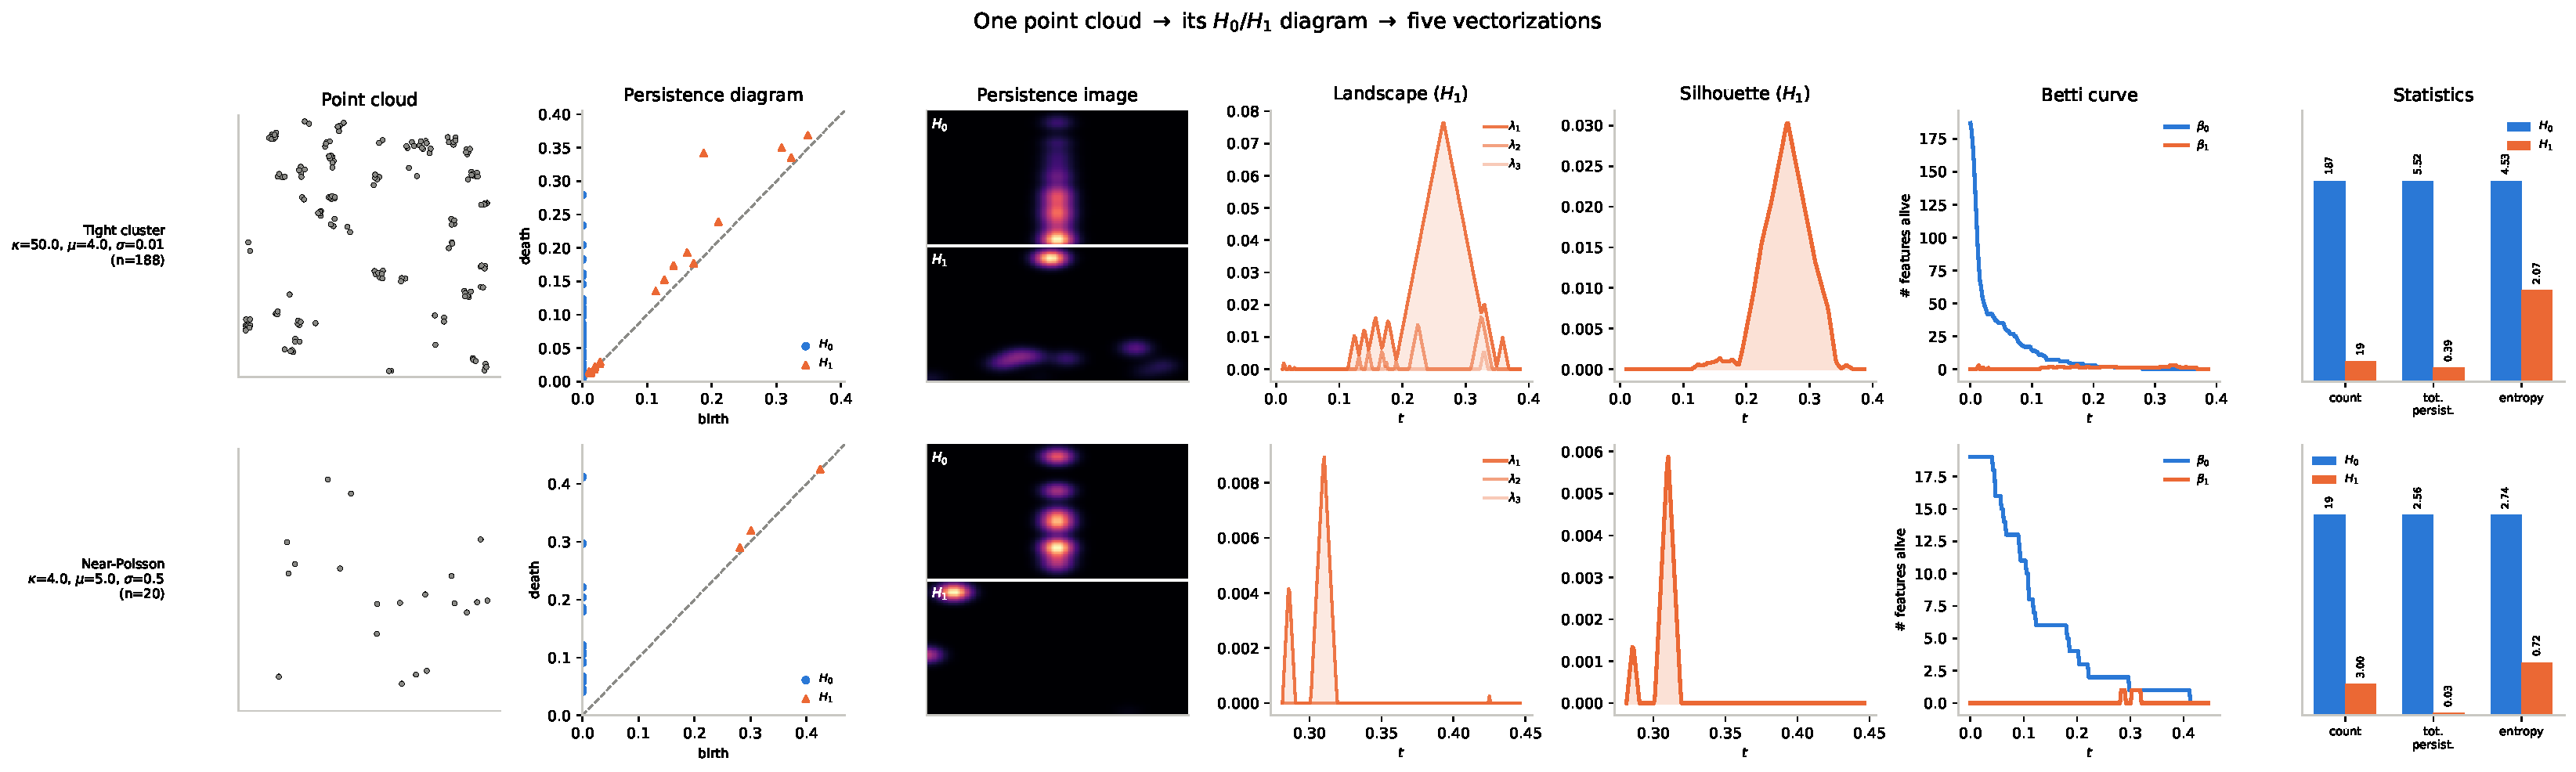
\includegraphics[width=\textwidth]{vectorization_schematic.pdf}
    \caption{One point cloud $\rightarrow$ its $H_0/H_1$ persistence diagrams
    $\rightarrow$ the five vectorizations compared in
    Section~\ref{ssec:exp-summaries}: persistence-image raster, landscape
    stack, silhouette curve, Betti curve, and persistence-statistics summary.
    Top row: the tight-cluster design ($\kappa=50$, $\mu=4$, $\sigma=0.01$);
    bottom row: the near-Poisson design ($\kappa=4$, $\mu=5$, $\sigma=0.5$),
    the same two extremes of Table~\ref{tab:sim-validation}. Statistics-panel
    bars are min-max normalized per statistic, with raw values printed above
    each bar, since count, total persistence, and entropy live on
    incomparable scales.}
    \label{fig:vectorization_schematic}
\end{figure}

% -----------------------------------------------------------------------------
\subsection{Background reading}
% -----------------------------------------------------------------------------
\todo{WRITE LAST. Reading clusters to cover:
 (a) classical SPP estimation -- Diggle, minimum contrast, Palm likelihood,
     composite likelihood;
 (b) TDA foundations -- persistence, stability, DTM filtrations;
 (c) vectorization of persistence -- persistence images, landscapes, Betti
     curves, kernel methods;
 (d) neural/simulation-based inference -- amortized inference, neural
     estimators, the two related works of Section 2;
 (e) TDA applied to point processes and to cosmology.}


% #############################################################################
% 4. PROBLEM SETUP
% #############################################################################

\section{Problem Setup}
\label{sec:problem}

Let $X$ be a Neyman-Scott process on $\R^d$ with unknown parameter vector
$\theta \in \R^{n_{params}}$. For example, the homogeneous Thomas process has 
$\theta = (\kappa, \mu, \sigma)$. We observe a single realization of $X$ on a 
bounded window $W \subset \R^d$, giving a point cloud
$\pc = \{x_1, \dots, x_n\} \subset \R^d$ with $n = |X \cap W|$. The objective is to 
produce an estimate $\hat\theta = \hat\theta(\pc)$ of $\theta$ from $\pc$ alone.
We stress \emph{single realization}: $\theta$ is not recovered from repeated draws of $X$, nor 
is $\pc$ pooled or averaged across realizations. This is the setting a practitioner
faces: one observed pattern and one chance to estimate the generating parameters.
It is also what makes the problem hard in a way no estimator can fix: a 
fixed $\theta$ already induces a distribution over point clouds, so even the true 
parameter value gives rise to a spread of plausible $\pc$, and it is this irreducible 
spread —- not any weakness of a particular estimator -— that sets the error floor 
characterized below.

The model is trained on a training set of synthetic clouds
$\{\pc_i, \theta_i\}_{i=1}^{N_{train}}$ by backpropagating the RMS loss
    \[
    \mathcal{L}(\hat\theta_i, \theta_i) = \sqrt{\sum_{j=1}^{n_{params}}(\hat\theta^j_i - \theta^j_i)^2},
    \]
where $\theta_i = (\theta_i^1, \dots, \theta_i^{n_{params}})$. Since parameters on a larger scale
dominate this loss, we train in log-normalized parameter space,
    \[
    \{\pc_i, \theta_i\}_{i=1}^{N_{train}} \rightarrow
    \left\{\pc_i, \frac{\log(\theta_i) - \mu_{\log\theta}}
    {\sigma_{\log\theta}}\right\}_{i=1}^{N_{train}},
    \]
where -- abusing notation -- $\mu_{\log\theta}, \sigma_{\log\theta}$ denote the
mean and standard deviation of the logged parameters.

We draw one realization per parameter vector. The dispersion of $\hat\theta$
across realizations sharing a common $\theta$ gives the irreducible error floor
against which the model's performance should be read.

\todo{make the error floor a named quantity here and reference it from
Section 7.3 -- it is the yardstick for every reported number}


% #############################################################################
% 5. SIMULATOR AND EXPERIMENTAL DESIGN
% #############################################################################

\section{Simulator and Experimental Design}
\label{sec:simulator}

Training data consists of pairs $(\pc_i, \theta_i)$ in which $\theta_i$ is drawn
from a design distribution $\Pi$ over parameters space and each $\pc_i$ is a
single realization of the corresponding process. We describe the design
distribution, sampling algorithm, and verification procedure used to generate
the synthetic data.

% -----------------------------------------------------------------------------
\subsection{Design distribution}
% -----------------------------------------------------------------------------

The naive approach of sampling $(\kappa, \mu, \sigma)$ uniformly and
independently from intervals is inadequate. Firstly, point processes can
typically be separated into qualitative regimes of interest, which occupy curved
subsets of the parameter grid. Therefore uniform sampling would allocate most of
its mass to configurations that are either near-Poisson or degenerate. Secondly,
the raw parameters are not comparable across families, for example Mat\'ern's
ball radius $R$ and Thomas's cluster scale $\sigma$ do not play equivalent roles.
We therefore sample in reparameterized coordinates that carry the same meaning
for every family considered:
    \begin{align*}
        \lambda &= \kappa\mu && \text{expected offspring intensity,} \\
        \kappa & && \text{parent intensity,} \\
        \nu &= r\sqrt{\kappa} && \text{dimensionless overlap index,}
    \end{align*}
where $r$ denotes the cluster scale of the family in question: $r = \sigma$ for
Thomas, $r = R$ for Mat\'ern cluster, and $r = \sqrt{\sigma_1^2 + \sigma_2^2}$
for nested Thomas. The overlap index $\nu$ measures cluster radius against mean
inter-parent spacing, so $\nu \ll 1$ gives well-separated clusters and
$\nu \gtrsim 1$ gives clusters that merge (so the process approaches complete
spatial randomness). Nested Thomas carries an additional coordinate, the scale
ratio $\rho = \sigma_2/\sigma_1 \in (0,1)$, which separates configurations in
which both levels of structure are resolvable from those in which the process
collapses to a single scale.

We draw $(\log\kappa, \log\lambda, \log\nu)$ uniformly over a grid and invert to
recover $\mu = \lambda/\kappa$ and $r = \nu/\sqrt{\kappa}$. Log-uniform sampling
is used because the parameters span several orders of magnitude, and it matches
the log-normalization applied to the ground-truth targets (see
Section \ref{sec:problem}) so that training targets are approximately uniform in
each coordinate. Draws are taken from a scrambled Sobol sequence.

The ranges of the design grid are constrained as follows:
    \begin{enumerate}
        \item \textbf{Point budget.} The cost of computing persistence summaries
        grows rapidly with the number of points, so we impose
        $\mathbb{E}[N] = \lambda \in [150, 800]$, fixing the range of
        $\log\lambda$.
        \item \textbf{Clusters per window.} We require $\kappa|W| = \kappa \geq 15$
        so that a single realization is informative about $\kappa$, and
        $\kappa|W| = \kappa \leq 120$ so that individual clusters remain
        resolvable.
        \item \textbf{Overlap.} We impose $\nu \in [0.10, 0.90]$. The upper
        limit deliberately admits the near-Poisson regime so that the model is
        still exposed to configurations in which the parameters are weakly
        identifiable.
    \end{enumerate}
Parameter draws violating these constraint are rejected and redrawn before any
cloud is generated. This filter acts on the design and not on realizations,
therefore it does not distort the conditional law of $\pc$ given $\theta$. The
realized acceptance rate is $24.8\%$.

% -----------------------------------------------------------------------------
\subsection{Sampling algorithm}
% -----------------------------------------------------------------------------

The various instances of a the Neyman--Scott construction may be generated by a
single algorithm. The only part that is different for each instance is the
displacement kernel $k$ and the offspring count distribution. For a window
$W \subset \R^d$:
    \begin{enumerate}
        \item Expand $W$ by an edge buffer $b$ to produce $W_{exp}$, so that
        clusters whose parents lie outside $W$ are not truncated.
        \item Sample the parent process on $W_{exp}$:
        $n \sim \mathrm{Poisson}(\kappa|W_{exp}|)$, with parents placed uniformly
        on $W_{exp}$.
        \item For each parent $p$ independently, draw an offspring count
        $n_p \sim \mathrm{Poisson}(\mu)$.
        \item For each offspring independently, draw a displacement
        $\epsilon \sim k$ and place the point at $p + \epsilon$.
        \item Discard the parents and retain the offspring lying in $W$.
    \end{enumerate}
For the Thomas process $k = \mathcal{N}(0, \simpcom^2 I_d)$; for the Mat\'ern
cluster process $k$ is uniform on the ball of radius $R$; for nested Thomas the
parent process at step 2 is itself a Thomas process rather than a homogeneous
Poisson process.

The buffer is set by a single rule applied to whichever kernel is in use: $b$ is
the radius containing all but $\varepsilon$ of the mass of $k$. For a Gaussian
kernel this gives $b = 4\sigma$, at which the per-axis tail mass is
$2\Phi(-4) \approx 6.3 \times 10^{-5}$; for the compactly supported Mat\'ern
cluster kernel it gives $b = R$ exactly, with no tail margin required; for nested
Thomas the buffers of the two levels add, giving $b = 4\sigma_1 + 4\sigma_2$,
which over-covers the tight bound $4\sqrt{\sigma_1^2 + \sigma_2^2}$ and is
therefore conservative. Points are never clipped to the boundary; the only
boundary operation is the containment filter at step 5.

% -----------------------------------------------------------------------------
\subsection{Validation}
\label{ssec:verification}
% -----------------------------------------------------------------------------

Throughout this section, let $X$ denote a point process on $\R^d$. We write
$u, v \in \R^d$ for points (precise locations) and $du$, $dv$ for infinitesimal
regions of volume $|du|$, $|dv|$ centered at $u$ and $v$, respectively.

    \begin{definition}[Second-order product density]
        The second-order product density
        $\rho^{(2)}: \R^d \times \R^d \rightarrow \R^+$
        is defined such that $\rho^{(2)}(u, v)\,du\,dv$ is the probability of
        jointly observing a point of $X$ in each of the infinitesimal regions
        $du$ and $dv$.
    \end{definition}

    \begin{definition}[Pair correlation function]
        The pair correlation function $g(u, v): R^d \times R^d \rightarrow \R^+$
        is defined
        \[
        g(u, v) = \frac{\rho^{(2)}(u, v)}{\rho(u)\rho(v)}.
        \]
    It is clear that for any Poisson process we have $g \equiv 1$. Intuitively,
    $g$ can suggest whether SPPs are attractive ($g > 1$), or repulsive
    ($g < 1$).
    \end{definition}

    \begin{definition}[Stationarity \& isotropy]
        A point process $X$ is said to be:
            \begin{itemize}
                \item \emph{Stationary} if $X \sim X + s$ for every
                $s \in \R^d$ where $X + s = \{x + s: x \in X\}$.
                \item \emph{Isotropic} if $X \sim RX$ for every rotation $R$
                about the origin.
            \end{itemize}
    \end{definition}

    \begin{note}
        Stationarity implies constant intensity $\rho(u) = \lambda$, but the
        converse is not necessarily the case. If $X$ is stationary and isotropic,
        $g(u, v)$ depends on $u$ and $v$ only through their inter-point distance
        $r = \|u - v\|$. Abusing notation, we may write $g(r)$ for this common
        value. We now define the $K$ function.
    \end{note}

    \begin{definition}[$K$-function]
        For stationary and isotropic $X$, the $K$-function
        $K(r): \R^+ \rightarrow R^+$ is defined
            \[
            K(r) = \int_{b_r(0)} g(\|h\|) dh
            \]
        Intuitively, $\rho(u)K(r)$ is the expected number of points we expect to
        see within a distance $r$ of a typical point in $X$.
    \end{definition}

% --- validation proper -------------------------------------------------------
Due to every downstream result being dependent on a diligent cloud-generation
process, we validate it against the established closed-form second-order theory.
On $W = [0,1]^2$ we compare $[[3000]]$ realizations at each of three parameter
triples spanning the design, chosen to span the overlap index: a tight-cluster
regime ($\nu = 0.07$), a moderate regime ($\nu = 0.22$), and a near-Poisson
regime ($\nu = 1.00$).
\todo{fix the $[[3000]]$ placeholder}

For the first moment, $\mathbb{E}[N(W)] = \kappa\mu|W|$. For the second, the
canonical identity $\mathrm{Var}[N(W)] = \kappa\mu(1+\mu)|W|$ holds only in the
limit of a window large relative to $\sigma$, and is badly biased in precisely
the near-Poisson regime we wish to stress. Applying the law of total variance to
$N(W) = \sum_p N_p(W)$ with
$N_p(W) \mid p \sim \mathrm{Poisson}(\mu q(p))$, $q(p) = \int_W k(x-p)\,dx$, and
evaluating the shot-noise term by Campbell's formula gives the exact
finite-window result
    \begin{equation}
    \label{eq:varN}
    \mathrm{Var}[N(W)] = \kappa\mu + \frac{\kappa\mu^2}{4\pi\sigma^2}J(\sigma)^2,
    \qquad
    J(\sigma) = \int_{-1}^{1}(1-|t|)\,e^{-t^2/4\sigma^2}\,dt,
    \end{equation}
for $W = [0,1]^2$, where the reduction to a one-dimensional integral follows from
the triangular density of the difference of two independent
$\mathrm{Uniform}(0,1)$ variables. As $\sigma \to 0$,
$J(\sigma) \to 2\sigma\sqrt{\pi}$ and \eqref{eq:varN} collapses to
$\kappa\mu(1+\mu)$, confirming the two agree in the appropriate limit. The gap
between them reaches $175\%$ at $\nu = 1$ (Figure~\ref{fig:variance_identity}),
so \eqref{eq:varN} is used as the comparison target.

\begin{figure}[h]
    \centering
    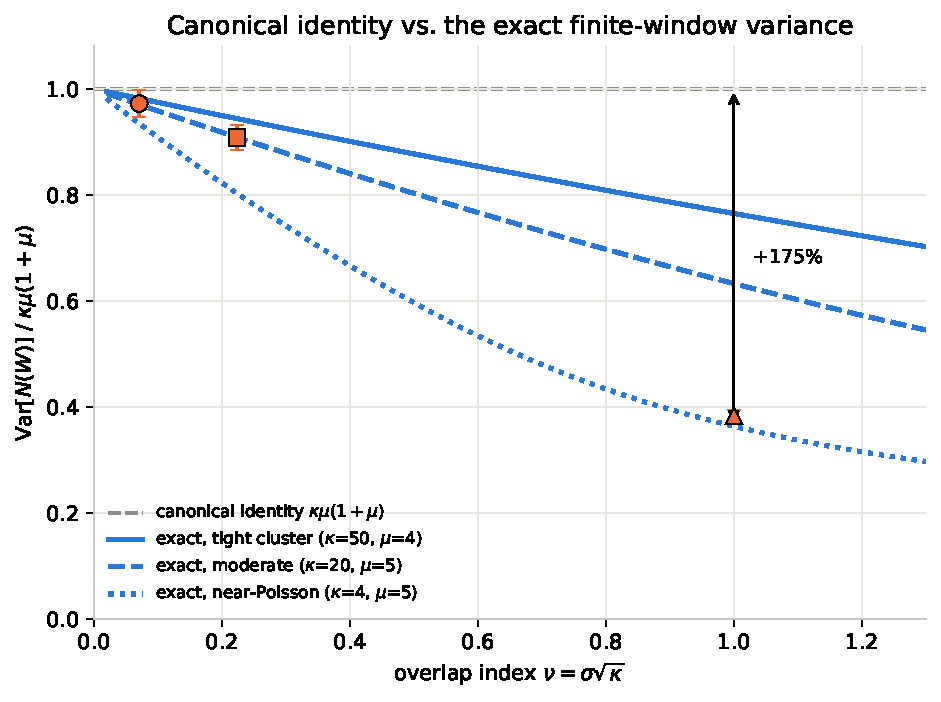
\includegraphics[width=0.72\textwidth]{variance_identity.pdf}
    \caption{The canonical identity $\mathrm{Var}[N(W)]=\kappa\mu(1+\mu)$
    (dashed reference, normalized to 1) against the exact finite-window
    result of \eqref{eq:varN}, as a function of the overlap index
    $\nu=\sigma\sqrt{\kappa}$, shown separately for each of the three
    validated designs of Table~\ref{tab:sim-validation} since the gap depends
    on $(\kappa,\mu)$ and not on $\nu$ alone. Markers are the empirical
    Monte Carlo variance at each design's own $\nu$ (mean $\pm$ 1 SE over
    $3000$ realizations), tracking the exact curve rather than the canonical
    line. At $\nu=1$ (near-Poisson design) the canonical identity
    overestimates the exact variance by $175\%$.}
    \label{fig:variance_identity}
\end{figure}

\begin{table}[h]
\centering
\begin{tabular}{lccccc}
\toprule
Case & $\nu$ & $\mathbb{E}[N]$ theory & empirical
     & $\mathrm{Var}[N]$ theory & empirical \\
\midrule
A & 0.07 & 200.0 & $200.4 \pm 0.6$ & 982.0 & $972.5 \pm 25.1$ \\
B & 0.22 & 100.0 & $100.2 \pm 0.4$ & 545.2 & $544.8 \pm 14.1$ \\
C & 1.00 & 20.0  & $20.0 \pm 0.1$  & 43.6  & $46.0 \pm 1.2$ \\
\bottomrule
\end{tabular}
\caption{Simulator validation against \eqref{eq:varN}. All deviations are within
$2$ standard errors.}
\label{tab:sim-validation}
\end{table}

We additionally verify that the empirical pair correlation function and Ripley's
$K$ match
    \[
    g(r) = 1 + \frac{e^{-r^2/4\sigma^2}}{4\pi\kappa\sigma^2},
    \qquad
    K(r) = \pi r^2 + \frac{1 - e^{-r^2/4\sigma^2}}{\kappa},
    \]
that the marginal offspring intensity on $W$ shows no boundary deficit
(edge-to-interior density ratio $1.003$--$1.048$ across the three cases, in all
cases consistent with unity and never in the direction an insufficient buffer
would produce), and that the displacement kernel is isotropic with per-axis
standard deviation matching $\sigma$. Estimates of $g$ normalized per realization
carry a negative bias that grows with $\mathbb{E}[N^2]$ and is therefore larger
for clustered patterns than for a matched-intensity Poisson control; we account
for this when reading residual deviations rather than attributing them to the
sampler.

% -----------------------------------------------------------------------------
\subsection{Splits and evaluation protocol}
% -----------------------------------------------------------------------------

Data are split by parameter vector, never by realization, so that no parameter
value appears in both training and evaluation. Beyond the random test split we
generate two further evaluation sets: a grid over the design grid, permitting
error to be reported as a surface over $(\log\nu, \log\lambda)$ rather than as a
single scalar; and a set drawn one increment outside each range, characterizing
degradation under extrapolation.

The classical baselines introduced in Section REF are run on the same clouds,
under the same train/test/grid/extrapolation splits rather than on separate data
or numbers taken from the literature. Section REF is therefore a comparison
against a shared  test set.

Throughout Section \ref{sec:experiments} we report error in the log-normalized
parameter space of Section \ref{sec:problem}. For a parameter vector with $n_{params}$
components and a test set of size $N_{test}$, we define the per-parameter loss
    \[
    \mathcal{L}^j = \frac{1}{N_{test}} \sum_{i=1}^{N_{test}}
    (\hat{\tilde\theta}^j_i - \tilde\theta^j_i)^2,
    \qquad
    \mathcal{L} = \frac{1}{n_{params}} \sum_{j=1}^{p} \mathcal{L}^j,
    \]
where $\tilde\theta$ denotes the log-normalized parameter vector and
$\hat{\tilde\theta}$ the model's estimate of it. Scalar figures quote
$\mathcal{L}$; where a single number obscures the behaviour of an individual
parameter we report the breakdown $\mathcal{L}^1, \dots, \mathcal{L}^{n_{params}}$
alongside it.

Two remarks. Firstly, $\mathcal{L}$ is the training objective of Section
\ref{sec:problem} up to the averaging over parameters and the square root, so
the quantity being optimized and the quantity being reported differ only in
scale; we report $\mathcal{L}$ rather than the training loss because the
per-parameter decomposition is not available from the latter. Secondly, because
the standardization is the one used at training time, $\mathcal{L}^j$ is
measured in units of the training-set variance of $\log\theta^j$. A value of
$\mathcal{L}^j = 1$ therefore corresponds to an error of one standard deviation
of $\log\theta^j$ over the design distribution, which is the error of a model
that has learned nothing beyond the mean of the design distribution. This gives
the upper reference point for every figure reported in Section
\ref{sec:experiments}; the lower reference point is the irreducible error floor
of Section \ref{sec:problem}.

We additionally report error in the original parameter units where a physical
reading is wanted, noting that these are not comparable across parameters and
are not the quantity being optimized.
\todo{confirm the reported figures in Section \ref{ssec:exp-ablations} are
$\mathcal{L}$ as defined here, and not the un-averaged training loss}


% #############################################################################
% 6. METHOD: PARAMNET
% #############################################################################
\section{Method: ParamNet}
\label{sec:method}

\expt{[none (log N only) | -- | -- | 5] and [PI | H0+H1 | DTM\{5,10,15\} | 5 |
log N removed]. Without these two the topological contribution is unquantified.}

Let $\pc$ denote a point cloud, $v$ its vectorized persistence summary, and
$e \in \R^{128}$ the resulting feature vector. ParamNet follows the pipeline
    \begin{equation}
    \label{eq:pipeline}
    \pc \xrightarrow{\;\text{Vectorization}\;} v
    \xrightarrow{\;\text{Encoder}\;} e
    \xrightarrow{\;\text{FCNN}\;} \hat\theta.
    \end{equation}

We note that the pipeline shape follows the neural-estimator patterns used in REF
and REF. Our contribution lies in the feature-extraction stage, the application to
a wider range of SPP families, and the careful evaluation of design choices.

The model is trained and evaluated on synthetic clouds generated by sweeping a
design distribution of the parameter space. The synthetic clouds are processed
together before training so that the feature-extraction step is performed only
once.

Feature extraction is the model's key component: it is where the cloud's 
topological summary is vectorized and made usable for machine learning. 
A substantial body of work has developed vectorizations of persistence 
diagrams —- persistence images, Betti curves, landscapes, kernel methods -- 
that trade off stability, resolution, and information loss in different ways, 
but there is little consensus on which is preferable for recovering 
generating parameters from a single observed point cloud. We implement and 
compare several such vectorizations against this task directly, rather than 
picking one on prior grounds; the comparison, and what it reveals about the 
structure each vectorization does and does not preserve, is the subject of 
Section~\ref{ssec:exp-summaries}.

The vectorized summary $v$ is passed through an encoder to obtain the
feature vector $e \in \R^{128}$, which is then given to the FCNN
$NN_\phi: \R^{128} \to \R^{n_params}$ to produce the estimate
$\hat\theta = (\hat\kappa, \hat\mu, \hat\sigma)$. $NN_\phi$ is a small feed-forward network: two hidden layers of width 64 and 
32, each followed by a ReLU nonlinearity and dropout ($p=0.1$), then a final 
linear layer mapping to the $n_{params}=3$ outputs $(\hat\kappa, \hat\mu, \hat\sigma)$.

% -----------------------------------------------------------------------------
\subsection{Filtration and vectorization}
% -----------------------------------------------------------------------------

\expt{Rips vs DTM claim still unsupported: [PI | H0+H1 | Rips | 5] against
[PI | H0+H1 | DTM\{5,10,15\} | 5]. Check the deficit concentrates in
$\kappa,\mu$ rather than $\sigma$ -- if it does not, the mechanism stated in
this subsection is wrong.}
\tab{Filtration comparison: Rips, DTM$_5$, DTM$_{10}$, DTM$_{15}$,
DTM$_{\{5,10,15\}}$. Columns: $\mathcal{L}$, per-parameter
$\mathcal{L}^\kappa,\mathcal{L}^\mu,\mathcal{L}^\sigma$, failed seeds.}

We describe the pipeline implemented for the
persistence image vectorization computed under the $DTM_k$ filtration, which is the
configuration carried through the rest of the paper. We give this configuration
in full because it is the most the one that raises design questions the alternatives do
not: the birth and persistence axes must be calibrated to a common frame before
the diagrams can be rasterized, and computing summaries at several values of $k$
leaves open how the resulting images are to be encoded and combined.

The pipeline is as follows;
    \begin{enumerate}
        \item Pick filtration function and construct filtrations
        $\{(\filt)_{r\geq 0}\}_i$.
        \item Compute persistence diagrams $\{D^{(0)}\}_i$, $\{D^{(1)}\}_i$.
        \item Calibrate diagrams to determine common birth/persistence axis
        ranges, shared across the dataset, then vectorize each diagram into a
        fixed-size raster using those ranges (see Definition
        \ref{def:per_image}).
    \end{enumerate}
The key design choices that follow are the filtration function, the calibration
procedure, and the image resolution. The latter two can be optimized with a
grid-search, but the choice of filtration function plays a fundamental role in
what information is available to be extracted at all. We use the $DTM_k$
filtration (see Example \ref{ex:dtm}) rather than the canonical Rips filtration.
Rips is built from inter-point distances alone, so it is sensitive to the
sparsest connection between two regions and does not register how densely those
regions are occupied, whereas $DTM_k$ averages over $k$ nearest neighbours and
so responds to local density directly. Since the parameters we wish to recover
are density parameters, we expect this to matter, and Section
REF reports the results that informed this decision.
Furthermore, the parameter $k$ allows us to compute summaries at various scales,
which may be combined to provide the model with a more complete picture that includes
both fine and coarse summaries.

Four alternative vectorizations -- landscapes, silhouettes, Betti/Euler curves, and
a persistence-statistics floor control -- are defined and compared in Section 
REF.

% -----------------------------------------------------------------------------
\subsection{Calibration}
\label{ssec:calibration}
% -----------------------------------------------------------------------------

\todo{Add one sentence: the coverage-quantile rule transfers unchanged to the
1-D grid calibration used by landscapes, silhouettes and Betti curves (Appendix
A). This is what makes the scheme a methodological contribution rather than a
persistence-image implementation detail.}

\expt{Calibration has no experiment attached to it anywhere. Minimum:
[PI | H0+H1 | DTM\{5,10,15\} | 3 | q $\in$ \{0.90,0.95,0.99,1.00\}], where
$q\to1$ recovers naive min/max, plus the train-only vs full-population leakage
arm.}

\fig{$\mathcal{L}$ against $q$ with $q=1.00$ marked as the naive endpoint.
One-parameter family, so this is a line plot, not a table.}
\fig{Naive vs coverage-quantile calibration applied to the same diagram, side
by side. The "loss of texture" argument is visual and is currently carried
entirely by prose.}

Consider the synthetic training clouds $\{\pc_i, \theta_i\}_{i=1}^{N_{train}}$
and fix the homology dimension $h \in \{0,1\}$ for some choice of filtration. We
obtain $N_{train}$ persistence diagrams $\{D^{(h)}_i\}_{i=1}^{N_{train}}$. Each
diagram will have a different distribution of points, some of which may have
extreme outliers with respect to the full set of diagrams.

In order to ensure that in the resulting persistence images each pixel bears the
same meaning, we calibrate the diagrams to have the same axis ranges. The
naive approach of calibrating to the maximum deaths and births (thus including all
points) is inadequate due to the resulting relative positioning of the
bulk of points: if we have a diagram with very strong outliers, the remaining diagrams
will be rescaled in a way that places the majority of their points near the origin. The diagrams -- and
therefore their vectorizations -- will lose a lot of texture
(Figure~\ref{fig:calibration_comparison}).

\begin{figure}[htbp]
    \centering
    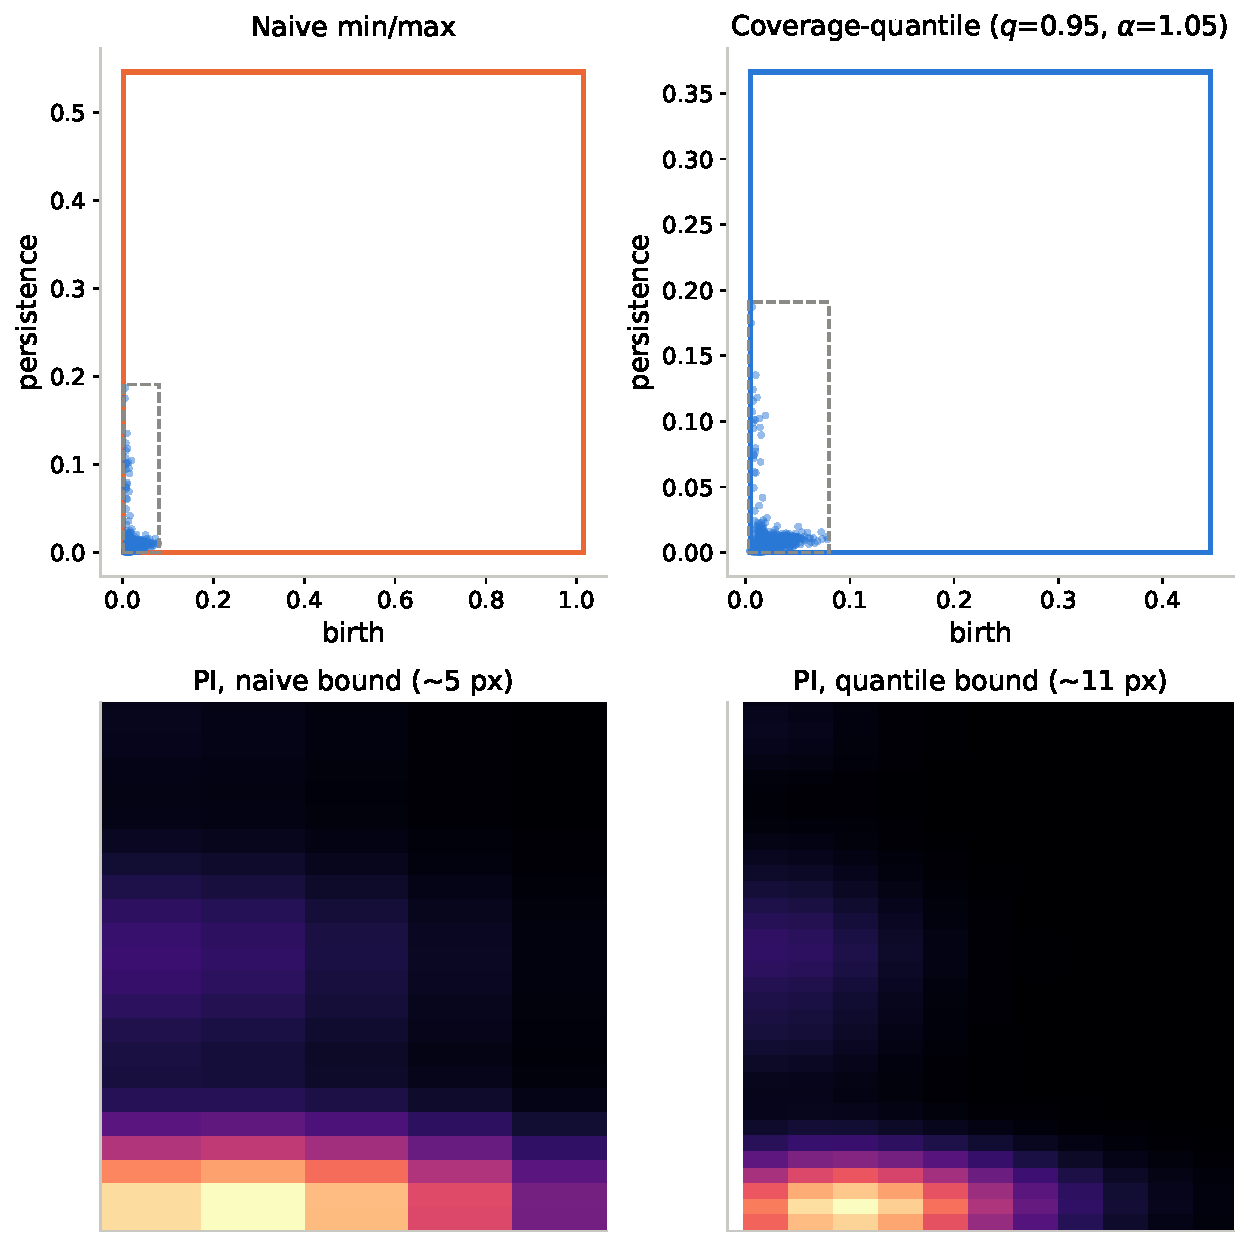
\includegraphics[width=0.85\textwidth]{calibration_comparison.pdf}
    \caption{The same $H_1$ diagram -- the population median by own max
    persistence, drawn from $1500$ clouds sampled from the production Thomas
    design distribution (Section~\ref{sec:simulator}) -- rendered under the
    naive pooled min/max bound (left) and the per-diagram coverage-quantile
    bound of $q=0.99$, $\alpha=1.05$ (right). Top row: the diagram's own
    points against the calibrated birth-persistence box; the naive box is
    stretched by a single high-offspring outlier diagram elsewhere in the
    population, not shown. Bottom row: the resulting persistence images --
    the same diagram occupies more of the frame, and its two close blobs
    stay resolved as separate texture, once the outlier is prevented from
    setting the shared axis range.}
    \label{fig:calibration_comparison}
\end{figure}

Our solution is to calibrate according to \emph{per-diagram coverage quantiles}.
For each training diagram $D_i^{(h)}$, define the three summary statistics
\begin{equation}
    b_i^{\min} = \min_{(b,d) \in D_i^{(h)}} b, \qquad
    b_i^{\max} = \max_{(b,d) \in D_i^{(h)}} b, \qquad
    p_i^{\max} = \max_{(b,d) \in D_i^{(h)}} (d - b),
\end{equation}
i.e. the smallest birth, largest birth, and largest persistence value attained
\emph{within a single diagram}. Given a coverage level $q \in (0,1)$ and a
padding factor $\alpha \geq 1$, we set the calibrated birth and persistence
ranges to be the $q$-quantiles of these per-diagram statistics, taken over the
training set:
\begin{equation}
    \big[\,Q_{1-q}\big(\{b_i^{\min}\}_{i=1}^{N_{train}}\big),\
    \alpha \cdot Q_{q}\big(\{b_i^{\max}\}_{i=1}^{N_{train}}\big)\,\big]
    \qquad \text{and} \qquad
    \big[\,0,\ \alpha \cdot
    Q_{q}\big(\{p_i^{\max}\}_{i=1}^{N_{train}}\big)\,\big],
\end{equation}
where $Q_q(\cdot)$ denotes the empirical $q$-quantile. In practice we take
$q = 0.99$ and $\alpha = 1.05$, which were determined via grid-search. These two
ranges are shared by every diagram of homology dimension $h$, for every point
cloud in the dataset (train, validation, test, and adversarial alike), so that a
given pixel of the resulting persistence image always refers to the same region
of birth-persistence space.

The key difference with the naive min/max calibration is \emph{what} is being
quantiled. Pooling all points from all diagrams and taking a quantile over that
pooled set implicitly weights each diagram by how many topological features it
produces: a single diagram with an unusually large number of points -- near the
diagonal or otherwise -- can dominate the resulting bound, while a diagram
consisting of one strong outlier and few other points contributes only that
outlier. By instead computing one representative statistic per diagram and
quantiling \emph{over diagrams}, every training cloud contributes exactly once to
the calibration, regardless of how many persistence pairs it happens to produce.
Framing outlier rejection as a coverage fraction over diagrams -- rather than
over points -- makes the trade-off explicit and controllable: at most
$\lceil (1-q) N_{train} \rceil$ diagrams may have their most extreme birth or
persistence value fall outside the calibrated frame (and are clipped rather than
discarded), while the bulk of the population retains full resolution. The naive
approach of calibrating to the global maximum is recovered as the degenerate case
$q \to 1$.

This scheme is also compatible with the stability guarantees of persistence
images \citep{adams2017persistence}, which are stated for a fixed bandwidth and a
fixed image domain: since $\sigma_{\text{pixels}}$ is specified in pixel units
(Definition \ref{def:per_image}) rather than in absolute birth/persistence units,
and the birth and persistence ranges are calibrated independently of one another,
a pixel remains a comparable, well-defined location across every image built from
the calibrated imager -- irrespective of the very different physical spans the
two axes typically have.

Because the calibrated ranges are a property of the training distribution, they
must be fit \emph{exclusively} on $\{D_i^{(h)}\}_{i \in \text{train}}$, then
frozen and applied unchanged to validation, test, and adversarial diagrams.
Fitting the ranges on the full, unsplit population of clouds -- before the
train/validation/test partition is drawn -- lets information about the held-out
clouds leak into the calibration used to build every training image, since every
pixel's meaning is defined relative to the calibrated bounds. As the
train/validation/test partition is redrawn per random seed, calibration must
likewise be refit per seed, on that seed's training rows only, and then applied
frozen to the corresponding validation, test, and adversarial rows.

For homology dimension $H_0$, birth values are often identically zero (or
otherwise carry negligible spread) under the chosen filtration, in which case
$b_i^{\min} \approx b_i^{\max}$ for all $i$ and the calibrated birth range
collapses to a point. We detect this case explicitly and fall back to a
one-dimensional vectorization of the diagram rather than fabricate an axis, since
a degenerate range would make an entire column of pixels convey no information.

% -----------------------------------------------------------------------------
\subsection{Encoder and fusion}
% -----------------------------------------------------------------------------

\expt{[PI | H0+H1 | DTM\{5,10,15\} | 5 | CoordConv removed]. Ideally crossed with
the calibration scheme -- the claim predicts CoordConv helps MORE under
calibrated axes than under naive ones, which would weld the two contributions
together.}

\expt{Multi-$k$ is the reason this subsection exists but is never justified:
[PI | H0+H1 | DTM\{5\} | 5], [PI | H0+H1 | DTM\{10\} | 5],
[PI | H0+H1 | DTM\{15\} | 5] against the fused arm.}

Consider the training clouds $\{\pc_i, \theta_i\}_{i=1}^{N_{train}}$. We pick $n_k$
scales for our $DTM_k$ filtration and compute persistence
images for $D$ homology dimensions with resolution $64 \times 64$.
So for batch size $B$, the encoding stage is comprised of the following
pipeline:
    \begin{align*}
    (B, n_k, D, 64, 64) \xrightarrow{\;\text{Processing}\;} (B\!\cdot\!n_k,D{+}2,64,64) \xrightarrow{\;\text{Encoder}\;} (B,n_k,E) \xrightarrow{\;\text{Fusion}\;} (B,3\!\cdot\!E+1)
    \end{align*}

During the processing step each $(D, 64, 64)$ persistence-image
stack is augmented with two coordinate channels -- fixed $x$- and
$y$-coordinate grids linearly spaced over $[-1, 1]$ -- following the CoordConv
construction \citep{liu2018coordconv}, so that the convolutional stack has access
to absolute pixel position rather than having to infer it. This ensures that the work
done during the calibration step is not lost: each pixel has a fixed,
shared meaning across the dataset and CoordConv lets the network exploit this
directly instead of relearning it.

To apply a shared encoder to all scales, the $n_k$-axis is folded into the
batch dimension for a single forward pass -- one call over $B \cdot n_k$ images
rather than $n_k$ separate calls -- so the weights are tied across scales by
construction rather than by an explicit sharing mechanism.

In the encoder stage, the coordinate-augmented tensor is then passed through a small
convolutional stack: three $3\times3$ convolution blocks with channel widths
$(32, 64, 128)$, each followed by a ReLU and $2\times2$ max-pooling with
spatial dropout between blocks (except the last one). The resulting
feature map is reduced by adaptive average pooling to a single spatial location
and projected by a linear layer to the embedding dimension $E$ to pruce a $(B, n_k, E)$ tensor.

The final step fuses the scales into a single feature vector of dimension $3\cdot E + 1$
by concatenating the $n_k$ embeddings along the feature axis and appending $\log N(\pc)$,
the logarithm of the number of points in the cloud. The resulting $(B, 3\cdot E + 1)$ tensor
is then passed to the FCNN head to produce the final parameter estimates.

A key design choice is whether to use a shared encoder across $k$-scales, or to use independent encoders
for each scale. Furthermore, the fusion step can also be done in several ways other than simple concatenation,
such as averaging or max-pooling the embeddings across scales.

We find that a shared encoder with concatenation is the best option (and also the simplest), and justify
this choice in Section REF by ablation studies.


% #############################################################################
% 7. EXPERIMENTS
% #############################################################################

\section{Experiments}
\label{sec:experiments}

\tab{Calibration sweep summary: swept parameter, values, selected value, and
the spread of $\mathcal{L}$ across the sweep. Compact -- it belongs here rather 
than in the appendix because it documents the selection procedure.}

Performing a grid search over all hyperparameters and architectures simultaneously is computationally infeasible, so
we adopt a greedy selection procedure. We begin by selecting the best architecture at a fixed default calibration,
then sweep the calibration parameters at the best architecture. Finally, we sweep vectorization-specific parameters 
with the best architecture and calibration fixed.

\subsection{Vectorization Comparisons}
\label{ssec:exp-summaries}

Figure~\ref{fig:vectorization_schematic} gives a visual overview of all five
vectorizations compared below, computed from the same persistence diagram.

\todo{Open with the DIAGNOSTIC framing, not the ranking. Three hypotheses,
stated before any numbers: (i) does raster/curve shape earn its keep over 18
order statistics (STAT floor control); (ii) does feature multiplicity matter
(landscape order statistics vs silhouette averaging); (iii) is the signed count
sufficient (Euler nested inside Betti). "PI wins" is one line and cannot carry
a section.}

\paragraph{Landscape.} The $K$ layers $\lambda_1(t) \geq \lambda_2(t) \geq
\dots \geq \lambda_K(t)$ are the order statistics of the tent family
$\{\Lambda_i(t)\}_i$ (Definition~\ref{def:tent}) at each grid point $t$:
$\lambda_j(t)$ is the $j$-th largest tent value. $K$ is chosen per diagram
sample by a coverage rule -- the smallest $K$ for which layer $K+1$ is
negligible for 99\% of training diagrams, capped at 16 -- giving a $(K,G)$
raster per homology dimension.

\paragraph{Silhouette.} Rather than keep every order statistic, the
silhouette collapses the same tents into one persistence-weighted average,
    \[
    \phi^{(p)}(t) = \frac{\sum_i |d_i-b_i|^p\, \Lambda_i(t)}
    {\sum_i |d_i-b_i|^p},
    \]
a single $(1,G)$ curve. $p=0$ is an unweighted mean over tents and $p \to
\infty$ concentrates entirely on the longest-lived feature; we run $p$ as an
arm over $\{0,1,2,3\}$.

\paragraph{Betti/Euler curve.} The Betti curve $\beta_k(r) = \#\{i : b_i
\leq r < d_i\}$ counts $k$-features alive at scale $r$ -- a feature count
rather than a tent reduction, but built from the same persistence pairs.
The Euler curve $\chi(r) = \beta_0(r) - \beta_1(r)$ is a signed count nested
inside the two Betti channels, not additional information.

\paragraph{Statistics.} The floor-control vectorization skips grids
entirely: 18 scalars per homology dimension -- count, total persistence,
persistent entropy, and the 10/25/50/75/90 quantiles of birth, death, and
lifetime -- computed directly from the finite pairs.

Full calibration (grid ranges, $K$-selection, shared vs.\ per-dimension
axes) and tensor shapes for all four are deferred to Appendix A.

\todo{Foreground the MLP control path early: every vectorization including the
persistence image is also run through the identical architecture-agnostic
\texttt{FlattenMLPEncoder}. If the ordering holds on both paths, the result is
about the summary and not the encoder. This is the strongest methodological
feature of the comparison and should not be buried.}

\expt{C1 native path, 8 arms $\times$ 5 seeds; C2 MLP path, 9 arms (incl.\ STAT)
$\times$ 5 seeds.}

\tab{MAIN COMPARISON. Rows = vectorization; columns = $\mathcal{L}$ (native),
$\mathcal{L}$ (MLP), per-parameter breakdown, vectorization dimension,
parameter count, failed seeds. The dimension column matters: PI at
$64\times64$ per (dim,scale) is 4096-d against a Betti curve's 128-d, and a
reader will otherwise assume the comparison was capacity-matched.}

\fig{Per-parameter error by vectorization, grouped bars, $\kappa/\mu/\sigma$.
This is the figure that carries the diagnostic claim -- the scalar table only
carries the ranking.}

\fig{Native vs MLP path scatter, one point per vectorization. Points near the
diagonal = the summary is doing the work; large vertical spread = the encoder is.}

\tab{Homology-dimension ablation (C3): PI, LS, BC $\times$ \{H0, H1, H0+H1\}.}

% -----------------------------------------------------------------------------
\subsection{Architecture ablations}
\label{ssec:exp-ablations}
% -----------------------------------------------------------------------------

\todo{Add one sentence stating this sweep was run on the persistence-image arm
at the default calibration, and that Section \ref{ssec:exp-summaries} confirms
persistence images are the arm worth ablating. Sequencing matters: had another
vectorization won, this subsection would describe a configuration the paper
does not ship.}

\tab{Full six-way encoder\_mode $\times$ fusion\_mode, promoted from the current
\texttt{center} environment to a proper table with caption and label.}

\fig{Per-seed loss scatter across the six configurations. The instability
finding is the interesting part and a table of means hides it.}

Experiments suggested that a shared encoder works just as well as the independent
option: we ran a sweep crossing \emph{encoder mode} (shared-weight vs.
independent-per-$k$) against \emph{fusion mode}, five seeds per combination, on
the same $DTM_{5,10,15}$ nested-Thomas setup used throughout. Restricting to the
simplest fusion strategy (flat concatenation), the shared-weight encoder matched
the independent one to within seed noise:

\begin{center}
\begin{tabular}{lccc}
\toprule
encoder mode & fusion & test loss (mean $\pm$ sd) & failed seeds \\
\midrule
shared      & concat & $0.200 \pm 0.009$ & $0/5$ \\
independent & concat & $0.217 \pm 0.028$ & $0/5$ \\
\bottomrule
\end{tabular}
\end{center}
\todo{promote to a proper \texttt{table} environment with a caption and label;
report the full six-configuration cross, not just the two concat rows}

with a ten-seed run of the shared-weight configuration ($0.205 \pm 0.012$)
confirming the same order of magnitude. Since tying weights across scales also
cuts the parameter count roughly $K$-fold and removes one design axis, we adopt
the shared encoder going forward.

% [MOVED FROM: old Section 3.3 -- fusion sweep]
We determined once again that the simplest option was the most effective, and we
concatenate the per-$k$ outputs. The full sweep, crossing both encoder mode and
fusion strategy (six combinations, five seeds each), showed that the two
convolutional-fusion variants are not simply worse on average but
\emph{unstable}: individual seeds collapse to a test loss of $\sim\!0.9$--$1.0$,
while other seeds of the very same configuration land right on the concatenation
baseline ($\sim\!0.20$).

Only the independent-encoder, flatten-pooled combination converged cleanly on all
five seeds, but even so it did not outperform plain concatenation
($0.212 \pm 0.005$ vs.\ $0.200 \pm 0.009$). Flat concatenation was therefore
preferred not only for its simplicity, but because it was the only strategy --
together with its shared/independent-encoder counterpart -- that trained reliably
across seeds without any sign of the collapse observed for the
convolutional-fusion alternatives.

\todo{FIGURE: per-seed test loss scatter across the six configurations. The
instability finding is the interesting part and a table of means hides it.}

% -----------------------------------------------------------------------------
\subsection{Estimation performance}
\label{ssec:exp-performance}
% #############################################################################

\paragraph{Comparison against classical estimators.}
\todo{minimum contrast on $K$ and on $g$, and Palm likelihood, run on the SAME
clouds (Section \ref{sec:simulator}). This is the headline comparison and the
only one that can substantiate the limitations claimed in Section 1.}

\paragraph{Error surfaces over the design grid.}
\todo{error as a surface over $(\log\nu, \log\lambda)$ using the grid evaluation
set. Expect degradation as $\nu \to 1$ (weak identifiability) -- if the model
degrades more gracefully than minimum contrast there, that IS the result.}

\paragraph{Per-parameter breakdown.}
\todo{$\kappa$, $\mu$, $\sigma$ separately. They are not equally hard and a
single scalar loss hides this.}

\paragraph{Performance relative to the irreducible error floor.}
\todo{report error as a ratio to the single-realization floor defined in
Section \ref{sec:problem}, so the numbers mean something absolute.}

\paragraph{Extrapolation.}
\todo{the out-of-range evaluation set -- degradation one increment outside each
design range.}

\paragraph{Cross-family results.}
\todo{Thomas / Mat\'ern cluster / nested Thomas. Whether one model trained across
families beats per-family models is an interesting question in itself, and the
common reparameterization of Section 5.1 is what makes it askable.}


% #############################################################################
% 8. DISCUSSION AND LIMITATIONS
% #############################################################################
% NOTE -- PURPOSE: pre-empt the obvious objections. Short.
% #############################################################################
\section{Discussion and Limitations}

\todo{Add a paragraph on the negative results: three alternative vectorizations
were implemented and none improved on persistence images. Say plainly what this
does and does not license -- it is evidence about these summaries under this
architecture and this design distribution, not a general claim about
vectorizations.}
\todo{Add: the per-diagram coverage rule was inherited unchanged by the 1-D
summaries for comparability, which may not be optimal for each individually.}
\tab{Compute cost: feature-extraction time per cloud by vectorization, training
time, and amortized inference time per cloud against minimum contrast per cloud.
The last comparison strongly favours the method and is currently unmentioned.}

\paragraph{The design distribution is a prior.}
% [MOVED FROM: end of old Section 3.1.4, where it was a stray closing remark]
Finally, we note that the design distribution acts as a prior, so the trained
model approximates a posterior summary under it, and its ranges must therefore
cover the intended application domain.
\todo{expand -- this is the single most important limitation of any amortized
estimator and deserves a full paragraph, not a trailing sentence}

\paragraph{Computational cost.}
\todo{persistence computation scales badly in $n$; this is why the point budget
of Section 5.1 is capped at 800. State the cost explicitly and compare against
the cost of minimum contrast.}

\paragraph{Single realization.}
\todo{the estimator sees one realization; classical methods often assume the
same, but say so explicitly}

\paragraph{Homogeneity and stationarity.}
\todo{everything here assumes homogeneous, stationary, isotropic processes}


% #############################################################################
% 9. FUTURE WORK
% #############################################################################
% NOTE -- PURPOSE: REQUIRED for the progression report; for the paper this can
% be folded into Section 8. Keep it concrete and sequenced -- this is the
% section the panel reads to judge whether there is a viable thesis here.
% #############################################################################
\section{Future Work}

\todo{immediate: complete Section \ref{ssec:exp-performance}. Give this a
timeline -- it is the nearest-term deliverable.}

\todo{near term: the encoder question flagged in Section 6.3 as requiring
further study -- attention over scales, set-based encoders operating on diagrams
directly rather than on rasters}

\todo{medium term: inhomogeneous / non-stationary processes, where classical
closed forms are least available and the topological approach has the most to
gain -- this is arguably where the thesis-scale contribution lies}

\todo{medium term: real data. Galaxy catalogues if the running example of
Section 1 is cosmological; name a specific dataset.}

\todo{longer term: uncertainty quantification -- the model currently emits a
point estimate with no interval, which limits its use as a drop-in replacement
for likelihood-based methods}


% #############################################################################
% BIBLIOGRAPHY
% #############################################################################
\todo{set up references.bib -- currently only \texttt{anai2020dtm},
\texttt{adams2017persistence}, and \texttt{liu2018coordconv} are cited, and the
Diggle / Tanaka references in Section 1 are inline text rather than citations}

\bibliographystyle{plainnat}
\bibliography{references}

\end{document}